\documentclass{report}
% Change "article" to "report" to get rid of page number on title page
\usepackage{amsmath,amsfonts,amsthm,amssymb}
\usepackage{setspace}
\usepackage{Tabbing}
\usepackage{fancyhdr}
\usepackage{lastpage}
\usepackage{extramarks}
\usepackage{chngpage}
\usepackage{soul,color}
\usepackage{listings}
\usepackage{enumerate}
\usepackage{graphicx,float,wrapfig}
\usepackage{pifont}
\usepackage{graphicx}
\usepackage[english]{babel}
\usepackage{tikz}
\usepackage[]{algorithm2e}
% In case you need to adjust margins:
\topmargin=-0.45in      %
\evensidemargin=0in     %
\oddsidemargin=0in      %
\textwidth=6.5in        %
\textheight=9.0in       %
\headsep=0.25in         %

\title{Assignment 1 - Comp 652 - Machine Learning}

% Homework Specific Information
\newcommand{\hmwkTitle}{Assignment 3}                     % Adjust this
\newcommand{\hmwkDueDate}{Tuesday, March 31 2015}                           % Adjust this
\newcommand{\hmwkClass}{COMP 652}


\newcommand{\hmwkClassInstructor}{Dr. Doina Precup}
\newcommand{\hmwkAuthorName}{Geoffrey Stanley}
\newcommand{\hmwkAuthorNumber}{260645907}
\newcommand{\Pp}{\mathbb{P}}
\newcommand{\Ev}{\mathbb{E}}
\newcommand{\cov}{\text{Cov}}
\newcommand{\Z}{\mathbb{Z}}
\newcommand{\R}{\mathbb{R}}
\newcommand{\dd}{\, \mathrm{d}}

% Setup the header and footer
\pagestyle{fancy}                                                       %
\lhead{\hmwkAuthorName}                              %
\chead{}
\rhead{\hmwkClass: \hmwkTitle}                                          %

\lfoot{}
\cfoot{}                                                                %
\rfoot{Page\ \thepage\ of\ \pageref{LastPage}}                          %
\renewcommand\headrulewidth{0.4pt}                                      %
\renewcommand\footrulewidth{0.4pt}                                      %

% This is used to trace down (pin point) problems
% in latexing a document:
%\tracingall
\definecolor{mygreen}{rgb}{0,0.6,0}
\lstset{commentstyle=\color{mygreen}, frame=single,  language=R, showspaces=false, showstringspaces=false}

%%%%%%%%%%%%%%%%%%%%%%%%%%%%%%%%%%%%%%%%%%%%%%%%%%%%%%%%%%%%%
% Make title
\title{\vspace{2in}\textmd{\textbf{\hmwkClass:\ \hmwkTitle}}\\
\normalsize\vspace{0.1in}\small{Due\ on\ \hmwkDueDate}\\
\vspace{0.1in}\large{\textit{Presented to \hmwkClassInstructor}}\vspace{3in}}
\date{}
\author{\textbf{\hmwkAuthorName}\\
    \textbf{Student ID: \hmwkAuthorNumber}}
%%%%%%%%%%%%%%%%%%%%%%%%%%%%%%%%%%%%%%%%%%%%%%%%%%%%%%%%%%%%%

\begin{document}
\maketitle
\section*{Question 1}
\subsection*{A)}
In the 4-neighbor spin glass model the maximal cliques were the edges between
each pixel. In an 8-neighbor spin glass model the maximal cliques become
clusters of 4 pixels. As such, parametization for a 4 neighbor spin glass model
will be as follows:

\begin{center}
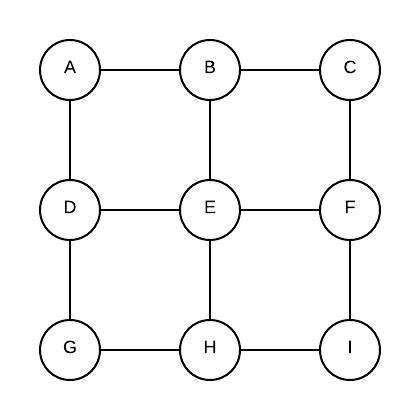
\includegraphics[width=125pt, keepaspectratio=true]{ising_model_4n.jpg}\\
\end{center}
\begin{equation}
  P(E) = \psi (B,E) \psi (D,E) \psi (E,F) \psi (E,H)
\end{equation}
While the parameters for an 8 neighbor spin glass model will be as such:
\begin{center}
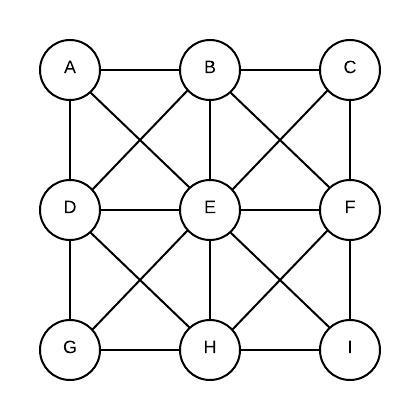
\includegraphics[width=125pt, keepaspectratio=true]{ising_model_8n.jpg}\\
\end{center}
\begin{equation}
  P(E) = \psi (A,B,D,E) \psi (B,C,E,F) \psi (D,E,G,H) \psi (E,F,H,I)
\end{equation}

\subsection*{B)}
The advantages and disadvantages would be related to a trade off between
model precision and computation time.\\

With the 8 neighbor model more data will be used to infer the value a pixel, this
could improve the models accuracy.This is at the expense of having to perform
more calculations as well as increasing the potential of overfitting the model.
\subsection*{C)}

\section*{Question 2}
\begin{center}
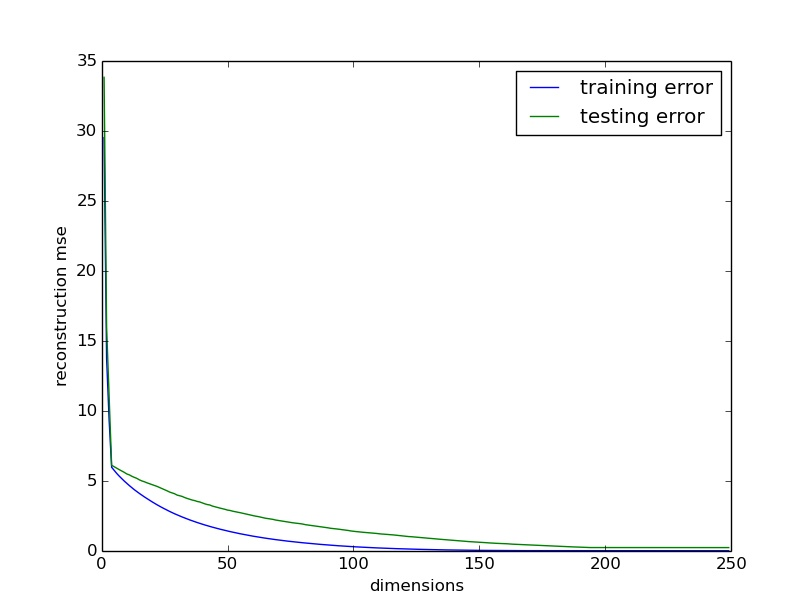
\includegraphics[width=250pt, keepaspectratio=true]{reconstruction_error.jpg}\\
\end{center}
As dimensions are reduced from 250 the reconstruction error is initially quite
small but becomes more important as dimensions approach 0. The
shoulder of the reconstruction error line is at a dimension of approximately 25.\\

From this, we can conclude that given this input space we can use PCA to
reduce dimensionality of the data to 25 in order to make computation more manageable
without losing very much granularity in the feature data.
\section*{Question 3}
\subsection*{A)}
As with standard Hidden Markov Models, Coupled Hidden Markov models will
have three categories of parameters. These are the initial probabilities, the
transition probabilites and the emission probabilities. Given the system
depicted in Figure 1 of assignment 3:\\

Initial Probabilities:
\begin{equation}
  P(s0)
\end{equation}
\begin{equation}
  P(u0)
\end{equation}\\

Transition Probabilities:
\begin{equation}
  P(s_i | s_{i-1}, u_{i-1})
\end{equation}
\begin{equation}
  P(u_i | u_{i-1}, s_{i-1})
\end{equation}\\

Emission Probabilities:
\begin{equation}
  P(y_i | s_i)
\end{equation}
\begin{equation}
  P(z_i | u_i)
\end{equation}

\subsection*{B)}
In order to compute the joint probability of a sequence of observations a
forward algorithm will need to be derived.


\begin{equation}
  \begin{aligned}
  \alpha_t(s_t, u_t) & = P(s_t, u_t, y_{0:T}, x_{0:T})\\
   & = \sum_{t-1 = 0}^T p(s_t, s_{t-1}, u_t, u_{t-1}, y_{1:T}, x_{1:T})\\
   & = \sum_{t-1 = 0}^T p(y_t | s_t) p(x_t | u_t) p(s_t | s_{t-1}, u_{t-1}) p(u_t | s_{t-1}, u_{t-1}) p(s_{t-1}, u_{t-1}, y_{1:T-1}, x_{1:T-1})\\
   & = \sum_{t-1 = 0}^T p(y_t | s_t) p(x_t | u_t) p(s_t | s_{t-1}, u_{t-1}) p(u_t | s_{t-1}, u_{t-1}) \alpha_{t-1}(y_{t-1}, x_{t-1})
  \end{aligned}
\end{equation}
\begin{equation}
  \alpha_0 (s_0, u_0) = p(y_0, z_0, s_0, u_0) = p(s_0) p(y_0 | s_0) p(u_0) p(z_0 | u_0)
\end{equation}

\subsection*{C)}

\begin{equation}
  \begin{aligned}
    \beta_k(s_k, u_k) & = p(y_{k+1:n} | s_k, u_k) p(z_{k+1:n} | s_k, u_k)\\
    & = \sum_{z_{k+1=1}}^m p(y_{k+1:n}, z_{k+1:n}, s_{k+1}, u_{k+1} | s_k, u_k)\\
    & = \sum_{z_{k+1=1}}^m p(y_{k+2:n} | s_{k+1}, u_{k+1}) p(z_{k+2:n} | s_{k+1}, u_{k+1}) p(y_{k+1} | s_{k+1}) p(z_{k+1} | u_{k+1}) p(s_{k+1} | s_k, u_k) p(u_{k+1} | s_k, u_k)\\
    & = \sum_{z_{k+1=1}}^m \beta_{k+1}(s_{k+1}, u_{k+1}) p(y_{k+1} | s_{k+1}) p(z_{k+1} | u_{k+1}) p(s_{k+1} | s_k, u_k) p(u_{k+1} | s_k, u_k)
  \end{aligned}
\end{equation}

\begin{equation}
  \beta_n (s_n, u_n) = 1
\end{equation}

\subsection*{D)}
The algorithm will remain largely the same except in the definition of the model
parameters. More specifically, the initial and transition probabilities will need
to be altered. K initial probabilities will be required and transition probabilities
would be defined as follows in the current model context:

\begin{equation}
  P(s_i | s_{i-k}, u_{i-k})
\end{equation}
\begin{equation}
  P(u_i | u_{i-k}, s_{i-k})
\end{equation}
\subsection*{E)}

\end{document}
